%!TEX root = ../Thesis.tex

\chapter{Auswertung und Ergebnisse}
\label{cha:results}

Die Stärken, Schwächen und Ergebnisse des entwickelten Algorithmus werden im nachfolgenden Kapitel
zusammengefasst, diskutiert und ausgewertet. Es wird zuerst abschnittsweise auf die drei primären Schritte
des Verfahrens eingegangen. Endergebnisse der Spurerkennung werden anschließend
in Form von Screenshots vorgestellt, in welchen die erkannten Fahrspuren zu sehen sind.

\section{Evaluierung der Datenvorverarbeitung}
\label{sec:results_eval_dataprocessing}

Die Datenvorverarbeitung ist ein wichtiger Teilschritt bei der Erkennung von Fahrspuren. Nur wenn aus
den Roh-Trajektorien die meisten Defekte entfernt wurden, können die nachfolgenden
Schritte zuverlässig funktionieren. Die angewandten Schritte zur
Entfernung der Anomalien sind in Abschnitt \ref{sec:realisation_preprocessing} beschrieben.
% Die Mehrzahl der Defekte in den Roh-Trajektoriedaten werden durch stehende
% Fahrzeuge und fehlerhafte oder unterbrochene Fahrzeugverfolgungen verursacht.

Dass die Entfernung von Ausreißern funktioniert, wurde bereits zum Teil in Abbildung
\ref{fig:real_result_2nd_Prepro} anhand des \textit{Neckartor}-Datensatzes gezeigt.
In Abbildung \ref{fig:results_prePro_heilbronner} sind nun die Trajektorien eines weiteren Datensatzes dargestellt,
welcher von der Heilbronner-Straße in Stuttgart stammt.

\begin{figure}[H]
    \centering
    \subfloat[]{{
        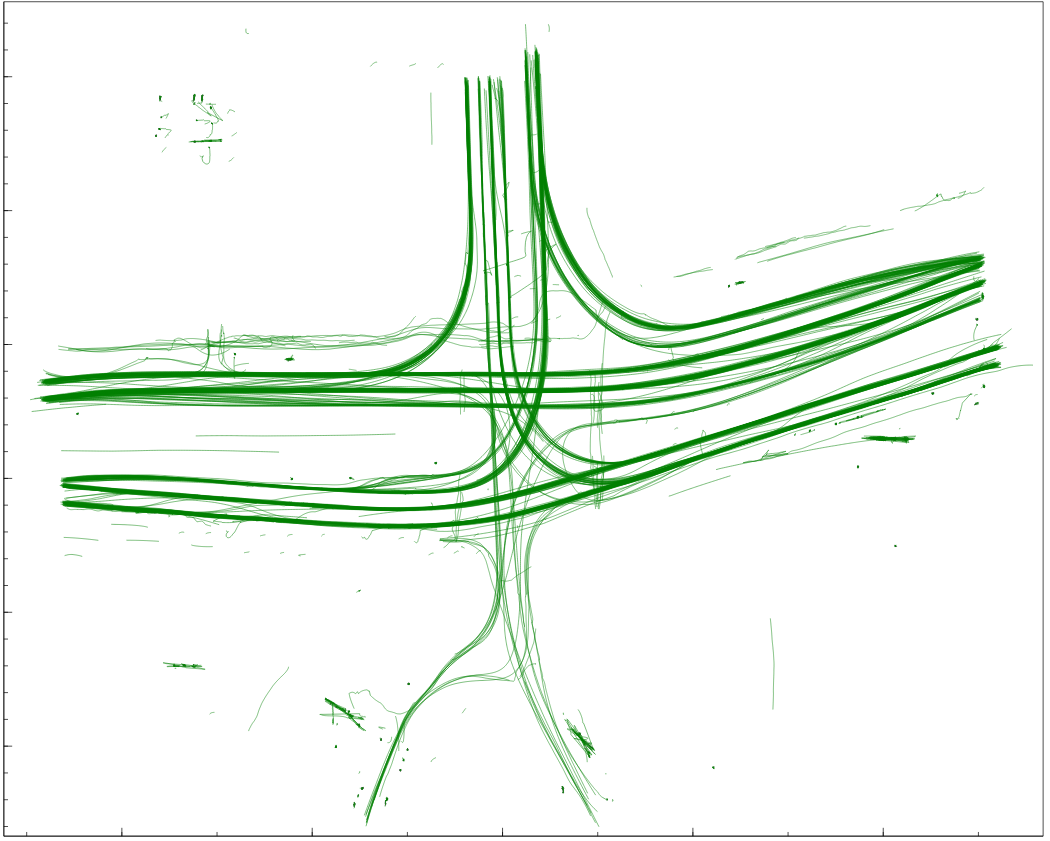
\includegraphics[align=c, width=0.33\linewidth]{resources/img/results/Heilbronner/rawTrajectories}
    }}
    \qquad \qquad
    \subfloat[]{{
        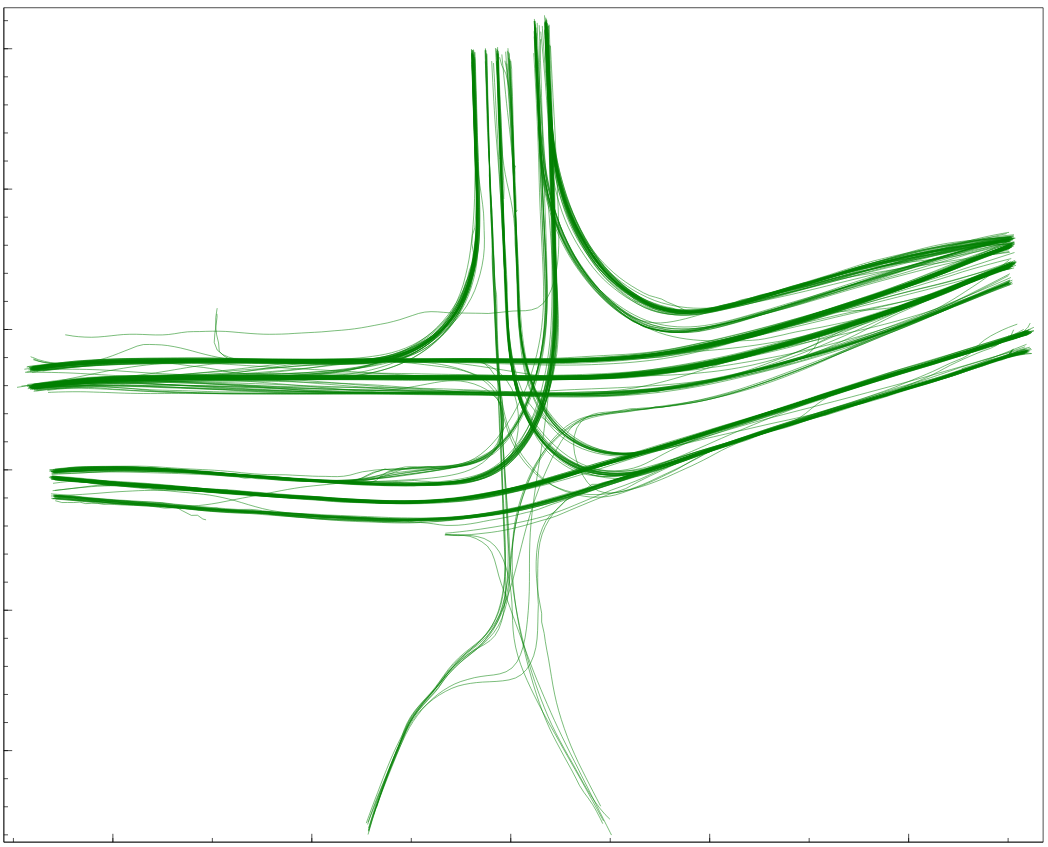
\includegraphics[align=c, width=0.33\linewidth]{resources/img/results/Heilbronner/preProTrajs}
    }}
    \caption{Ergebnis Vorverarbeitung Heilbronner-Straße}
    \label{fig:results_prePro_heilbronner}
\end{figure}

Die zwei obigen Plots zeigen gut, dass die vielen in a) vorkommenden Ausreißer entfernt wurden. Von den
circa 1050 Roh-Trajektorien im ursprünglichen Datensatz bleiben nach der Vorverarbeitung etwa 450 intakte
Bewegungsbahnen übrig. Die Mehrzahl der Defekte in diesem Fall stammt von fehlerhaften Objekterkennungen
und unterbrochener Fahrzeug-Detektionen, welche aufgrund der Verdeckung von Fahrspuren durch Bäume entstehen.

Ein problematisches Verhalten des Vorverarbeitungsschrittes wurde beim Testen der Spurerkennung anhand eines
Datensatzes aus Steinheim deutlich. In Abbildung \ref{fig:results_horizon_problem} a) ist der
untersuchte Straßenabschnitt dargestellt.

\begin{figure}[H]
    \centering
    \subfloat[]{{
        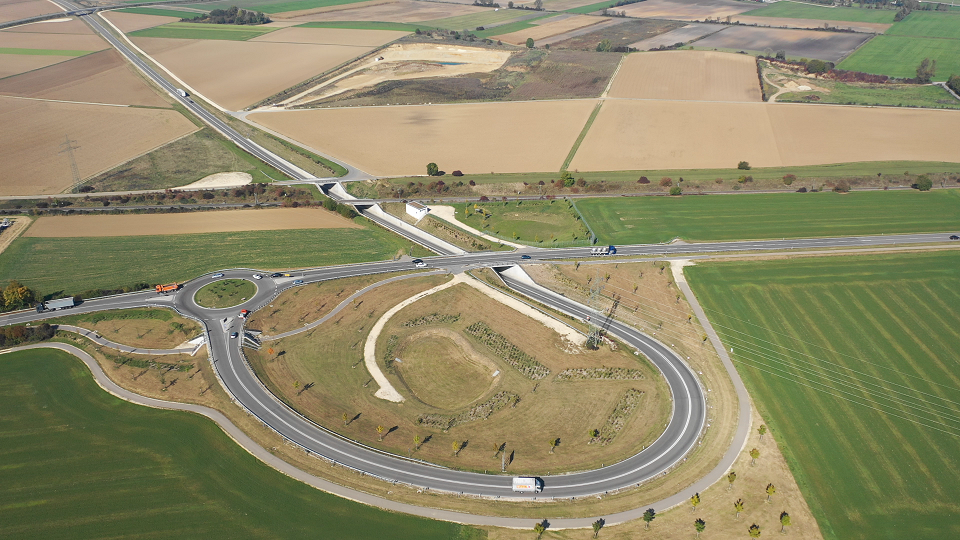
\includegraphics[align=c, width=0.35\linewidth]{resources/img/results/Steinheim/steinheim}
    }}
    \qquad \qquad \qquad
    \subfloat[]{{
        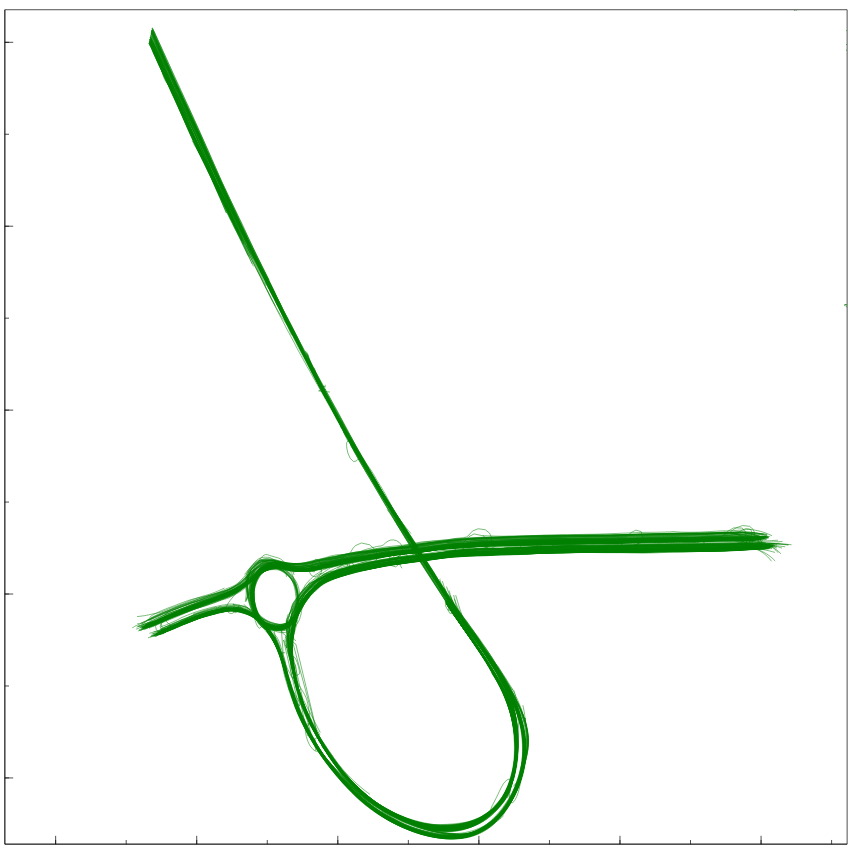
\includegraphics[align=c, width=0.25\linewidth]{resources/img/results/Steinheim/preProTrajs_cut}
    }}
    \caption{Straßenausschnitt Steinheim a), gekürzte Trajektorien b)}
    \label{fig:results_horizon_problem}
\end{figure}

Kritisch an dieser Aufnahme ist, dass die Fahrzeuge, welche sich auf der oben links startenden Fahrbahn bewegen,
am Anfang beziehungsweise Ende ihrer Fahrt sehr klein sind. Da Fahrzeuge in einer Aufnahme ab einer gewissen Größe
nurnoch sehr unzuverlässig detektiert werden, brechen die Trajektorien in diesem Fall auf sehr
unterschiedlichen Höhen ab.
Problematisch ist nun, dass der in Abschnitt \ref{sec:real1_remove_broken_trajectories} beschriebene Algorithmus
zur Entfernung unterbrochener Trajektorien, aufgrund der stark variierenden Start- und End-Positionen,
auch die meisten Trajektorien auf der nach hinten verlaufenden Fahrbahn entfernt und somit die Spuren
nicht erkannt werden können. Dieses Verhalten kann immer dann auftreten, wenn Fahrbahnen auf einen
von der Kamera weit entfernten Horizont zulaufen.

Da Fahrzeuge im Bereich eines solchen Horizonts grundsätzlich unzuverlässig erkannt werden, ist auch eine Fahrverhaltensanalyse
mithilfe von Fahrspuren hier nicht sinnvoll. Es wurde daher entschieden, dem Anwender die Möglichkeit zu geben, eine
Horizont-Linie zu definieren. In einem ersten Vorverarbeitungsschritt werden alle Trajektorie-Punkte oberhalb dieser
Linie entfernt. Das Ergebnis dieses Verfahrens ist in Abbildung \ref{fig:results_horizon_problem} b)
dargestellt. Dank der Beschneidung der Trajektorien bleiben diese in den nachfolgenden Verarbeitungsschritten
erhalten und es können Spuren im gewünschten Ausschnitt erkannt werden.

Mit Ausnahme des unerwünschten Verhaltens im Fall von Trajektorien, welche am Horizont sehr unterschiedliche Start-
beziehungsweise End-Positionen besitzen, funktioniert die Datenvorverarbeitung zuverlässig und wie gewünscht.
Voraussetzung dafür, dass nach der Datenvorverarbeitung
noch genug Trajektorien vorliegen welche weiterverarbeitet werden können, ist, dass in
den Rohdaten genügend intakte, vollständige Bewegungsbahnen vorhanden sind.

\section{Evaluierung der Clusteranalyse}
\label{sec:results_eval_clustering}

Die Clusteranalyse der Trajektorien bildet die Grundlage für die anschließende Bestimmung der Spur-Geometrien.
Sie ist daher ein kritischer Bestandteil der Spurerkennung. Der in dieser Arbeit eingesetzte Ansatz zur
Gruppierung der Trajektorien wurde in Abschnitt \ref{sec:real_ansatz_dbscan_lcss} beschrieben.
Hier wurden auch bereits Ergebnisse der Clusteranalyse für die Datensätze \textit{Entennest} und
\textit{Neckartor} vorgestellt.

Da der angewandte Clustering-Algorithmus die vollständigen Verläufe der
Trajektorien vergleicht, ist die wichtigste Vorraussetzung zur Identifikation eines Clusters, dass ausreichend
Trajektorien vorliegen, welche die identische Bewegung durch einen Straßenabschnitt beschreiben.
In Abschnitt \ref{sec:results_clustering_dbscan_lcss} wurde erwähnt, dass ein Cluster mindestens aus
fünf Trajektorien bestehen muss. Diese Untergrenze wurde gewählt, um nicht zu viele Cluster zu finden, welche
eigentlich keine Fahrspur beschreiben. Würde die Grenze niedriger angesetzt werden, so würden beispielsweise
vermehrt Cluster aus Trajektorien gebildet, welche Überholvorgänge beschreiben.

In den meisten Datensätzen anhand derer der in dieser Arbeit entwickelte Algorithmus getestet wurde,
existierten ausreichend Trajektorien pro Fahrspur, um diese zuverlässig zu identifizieren. Eine Ausnahme
stellt der Datensatz von der Heilbronner-Straße in Stuttgart dar, dessen Trajektorien bereits
in Abschnitt \ref{sec:results_eval_dataprocessing} dargestellt sind. In Abbildung \ref{fig:results_prePro_heilbronner} b)
wird deutlich, dass die Fahrspuren im
unteren Bereich des Straßenabschnitts nur wenig befahren sind. Dies wirkt sich auch auf das Ergebnis
der Clusteranalyse aus, welches in Abbildung \ref{fig:results_clusters} a) dargestellt ist.
Zwar existieren ausreichend Trajektorien, welche sich von oben nach unten links bewegen, allerdings können
keine Cluster aus den Trajektorien gebildet werden, welche sich unten rechts befinden.
Die wenigen in diesem Bereich existierenden Trajektorien haben sehr unterschiedliche Bewegungsbahnen,
weshalb hier kein Cluster identifiziert wird.

\begin{figure}[H]
    \centering
    \subfloat[]{{
        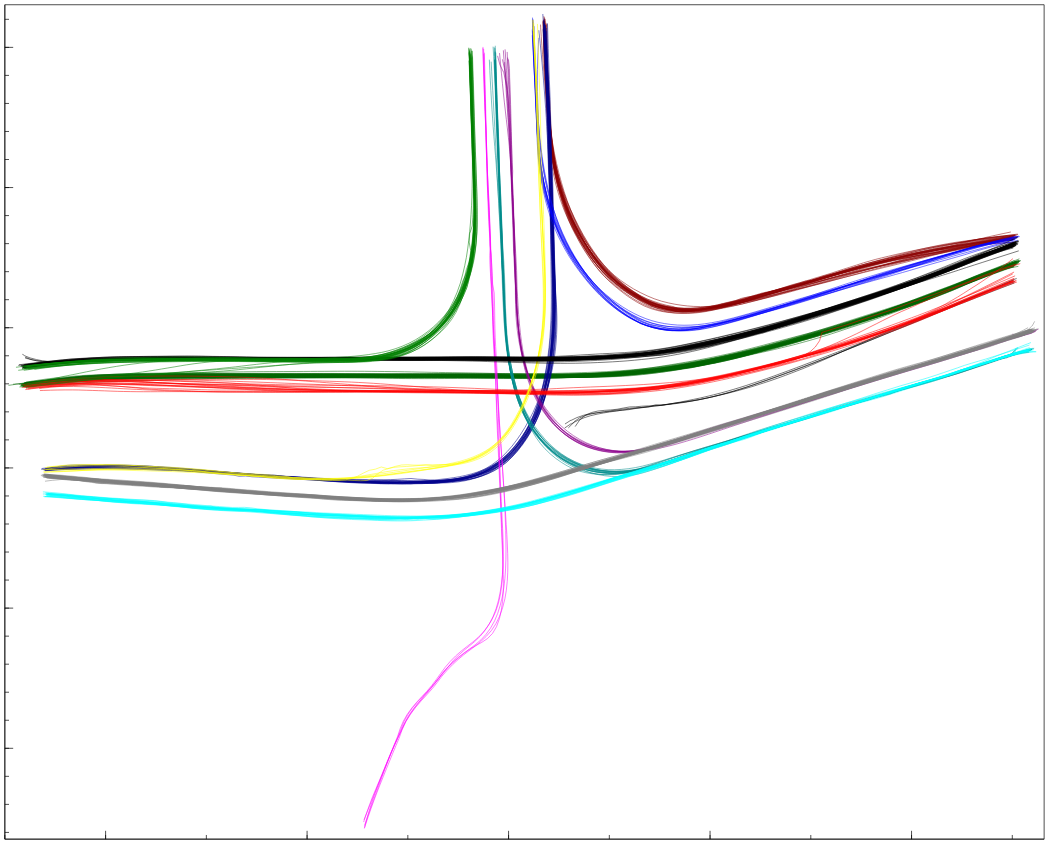
\includegraphics[align=c, width=0.31\linewidth]{resources/img/results/Heilbronner/filteredClusters_Heilbronner}
    }}
    \subfloat[]{{
        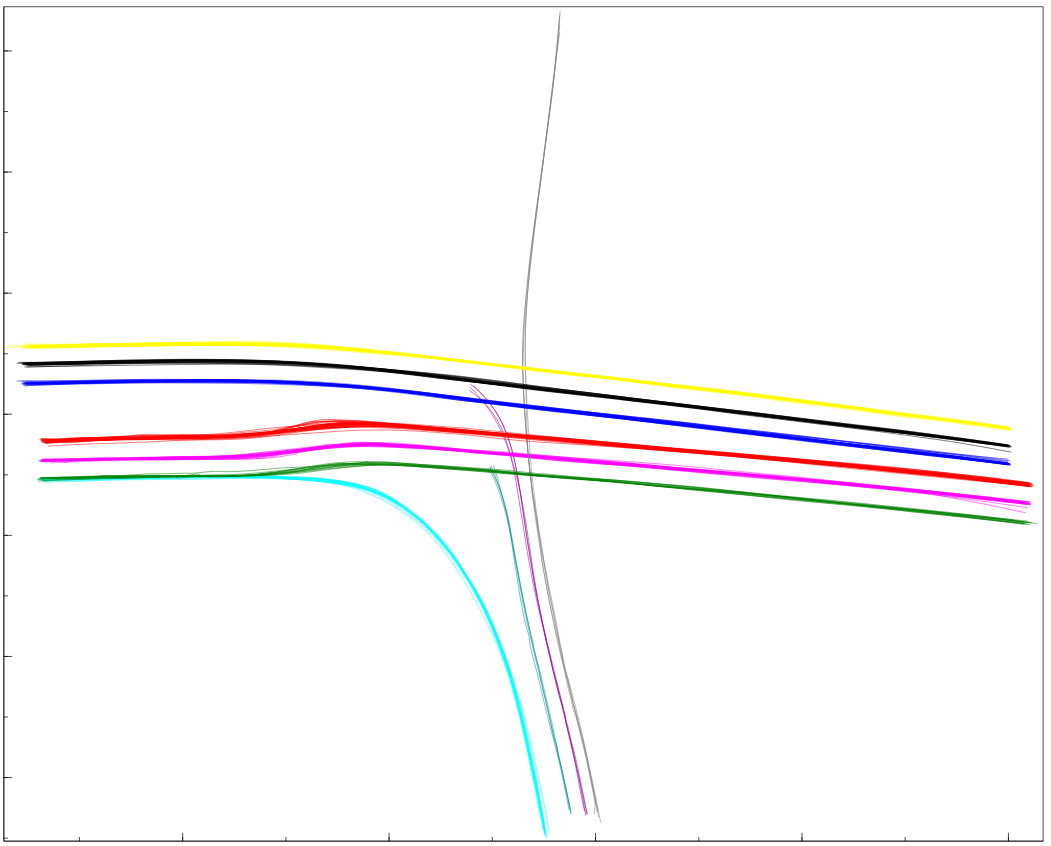
\includegraphics[align=c, width=0.31\linewidth]{resources/img/results/Neckartor/filteredClusters1}
    }}
    \subfloat[]{{
        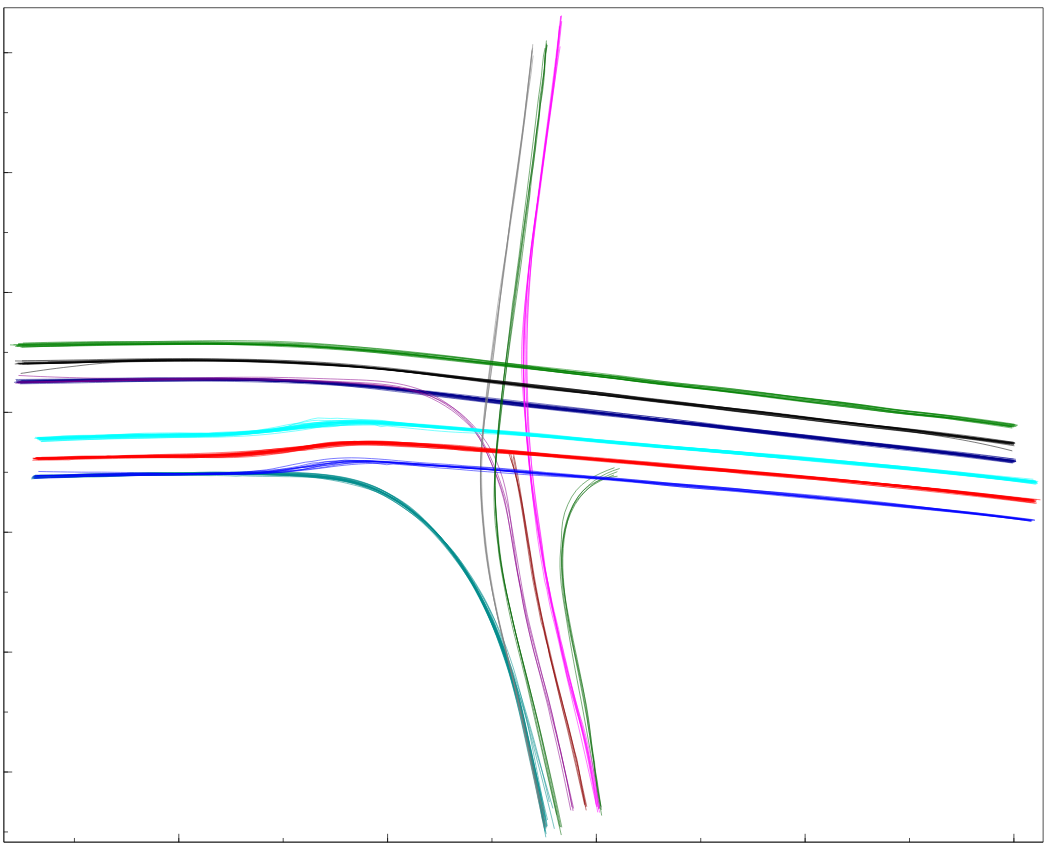
\includegraphics[align=c, width=0.31\linewidth]{resources/img/results/Neckartor/filteredClusters2}
    }}
    \caption{Trajektorie-Cluster Heilbronner-Straße und Neckator-Kreuzung}
    \label{fig:results_clusters}
\end{figure}

Die Plots in Abbildung \ref{fig:results_clusters} b) und c) zeigen das Ergebnis der Clusteranalyse für
den \textit{Neckartor}-Datensatz, aus welchem vor Anwendung des Algorithmus zufällig 50\% der Trajektorien entfernt wurden.
Auch hier wird deutlich, dass das Ergebnis maßgeblich von der Anzahl der Trajektorien pro Spur abhängt.
In Plot b) wurden viele vertikal verlaufende Trajektorien entfernt, weshalb hier nur wenige Spurcluster identifiziert werden.
In Plot c) wurden hingegen, trotz des Fehlens von 50\% der Trajektorien, fast alle Spurcluster erkannt
(vergleiche Abbildung \ref{fig:real_turning_lane} c)).

Außer von der Anzahl der Trajektorien hängt das Ergebnis der Clusteranalyse maßgeblich von den gewählten
Parametern des DBSCAN Algorithmus und des LCSS Distanzmaßes ab. Die in Abschnitt \ref{sec:results_clustering_dbscan_lcss} definierten
Standardparameter liefern in der Mehrzahl der Fälle gute Ergebnisse. Alle oben dargestellten Plots
wurden mit diesen Parametern erstellt.
Anderer Parameter müssen lediglich dann gewählt werden, wenn sich die Trajektorien unterschiedlicher
Fahrspuren in einer Aufnahme stark überlagern.
Dies ist beispielsweise im Datensatz \textit{Düsseldorf} der Fall, da sich hier eine Fahrspur nach circa 400 Metern in drei Spuren unterteilt.
Die Trajektorien des Datensatzes sind in Abbildung \ref{fig:results_clusters_duesseldorf} a) dargestellt.
Um sie klar in Spurcluster unterteilen zu können, muss statt dem Standardwert
$\epsilon_{DBSCAN} = 0.3$ der Wert $\epsilon_{DBSCAN} = 0.1$ verwendet werden. Das Ergebnis der Clusteranalyse
unter Einsatz dieses Parameters ist in Abbildung \ref{fig:results_clusters_duesseldorf} b) zu sehen.

\begin{figure}[H]
    \centering
    \subfloat[]{{
        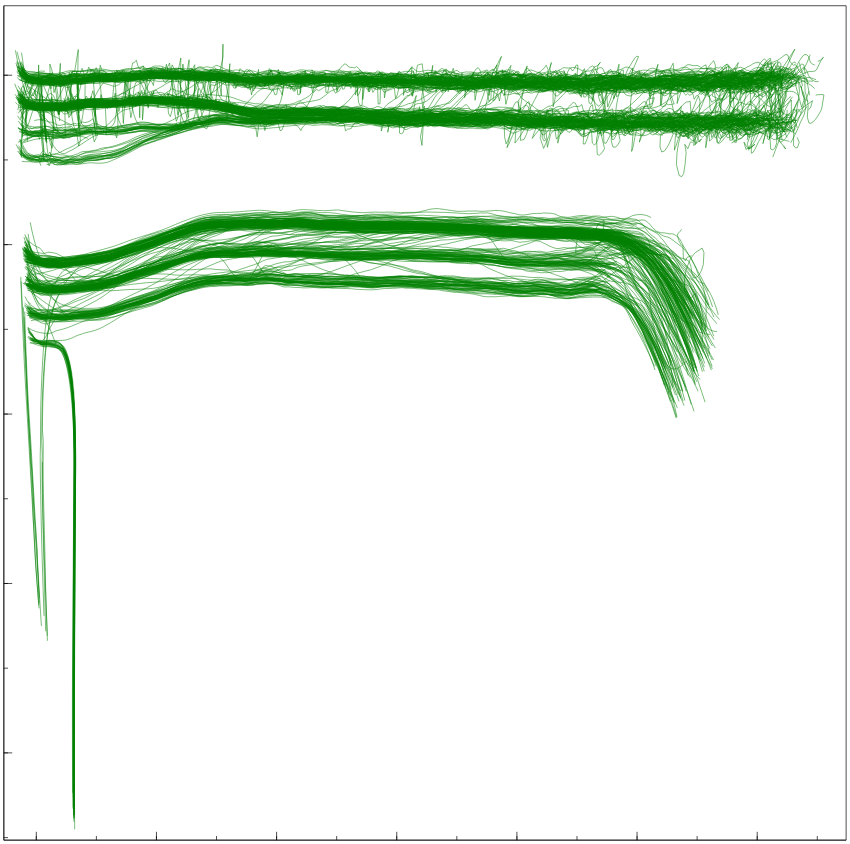
\includegraphics[align=c, width=0.31\linewidth]{resources/img/results/Duesseldorf/preProTrajs}
    }}
    \qquad \qquad
    \subfloat[]{{
        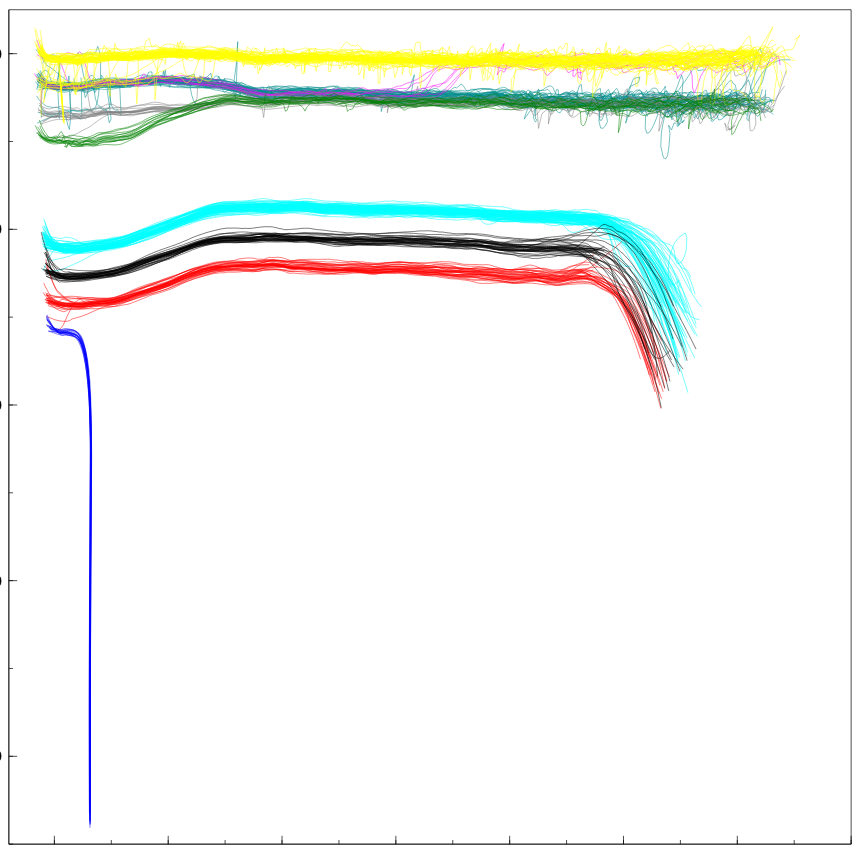
\includegraphics[align=c, width=0.31\linewidth]{resources/img/results/Duesseldorf/filteredClusters_Duesseldorf}
    }}
    \caption{Trajektorien Düsseldorf Datensatz a), Spurcluster b)}
    \label{fig:results_clusters_duesseldorf}
\end{figure}

Die Verwendung des alternativen Wertes für $\epsilon_{DBSCAN}$ liefert in Fällen, in welchen sich Spuren stark überlagern,
gute Resultate. Um das Verhalten des Algorithmus in dieser Hinsicht steuern zu können, wurde dem Nutzer die Möglichkeit
gegeben, $\epsilon_{DBSCAN}$ beim starten des Spurerkennungs-Jobs anzupassen.

Für die Clusteranalyse kann zusammenfassend festgehalten werden, dass sie gut funktioniert, wenn ausreichend Trajektorien
zur Beschreibung einer Spur vorliegen. Ihr Verhalten kann bei Bedarf zudem angepasst werden.

\section{Evaluierung der Spur-Geometrie-Bestimmung}

Nach der Clusteranalyse werden anhand der identifizierten Trajektoriecluster die Geometrien der Fahrspuren
bestimmt. Ziel dieses Schrittes ist es, Spur-Geometrien zu definieren, welche den realen Spur-Abmaßen möglichst
genau entsprechen. Die angewandten Verfahren sind in Abschnitt \ref{cha:lane_definition} beschrieben.

Wurden im vorherigen Schritt Trajektorie-Cluster für die in einer Aufnahme enthaltenen Spuren identifiziert,
so können auf Basis dieser meist zuverlässige Spur-Geometrien abgeleitet werden.
In Abbildung \ref{fig:results_laneGeometries} sind beispielhaft Spurgeometrien aus drei unterschiedlichen Datensätzen dargestellt.

% TODO: Update Plot Steinheim
\begin{figure}[H]
    \centering
    \subfloat[Heilbronner-Straße]{{
        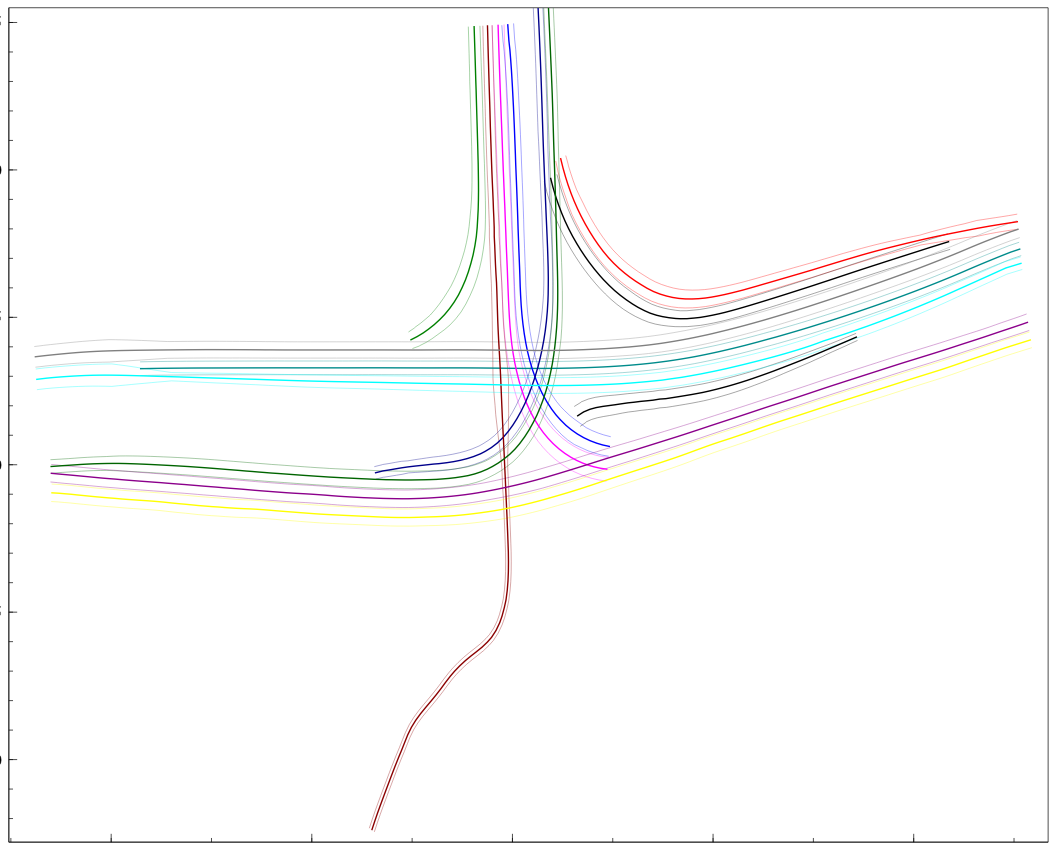
\includegraphics[align=c, width=0.29\linewidth]{resources/img/results/Heilbronner/improvedLanes_Heilbronner}
    }}
    \subfloat[Düsseldorf]{{
        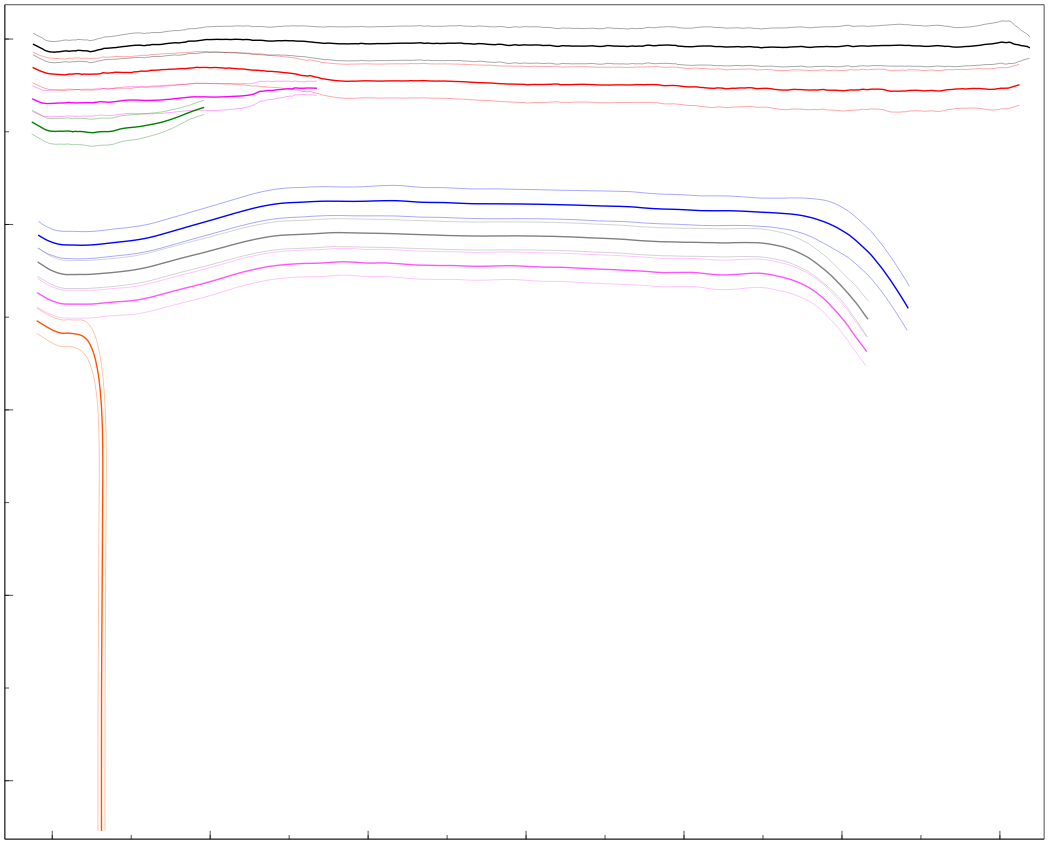
\includegraphics[align=c, width=0.29\linewidth]{resources/img/results/Duesseldorf/improvedLanes_Duesseldorf}
    }}
    \subfloat[Steinheim]{{
        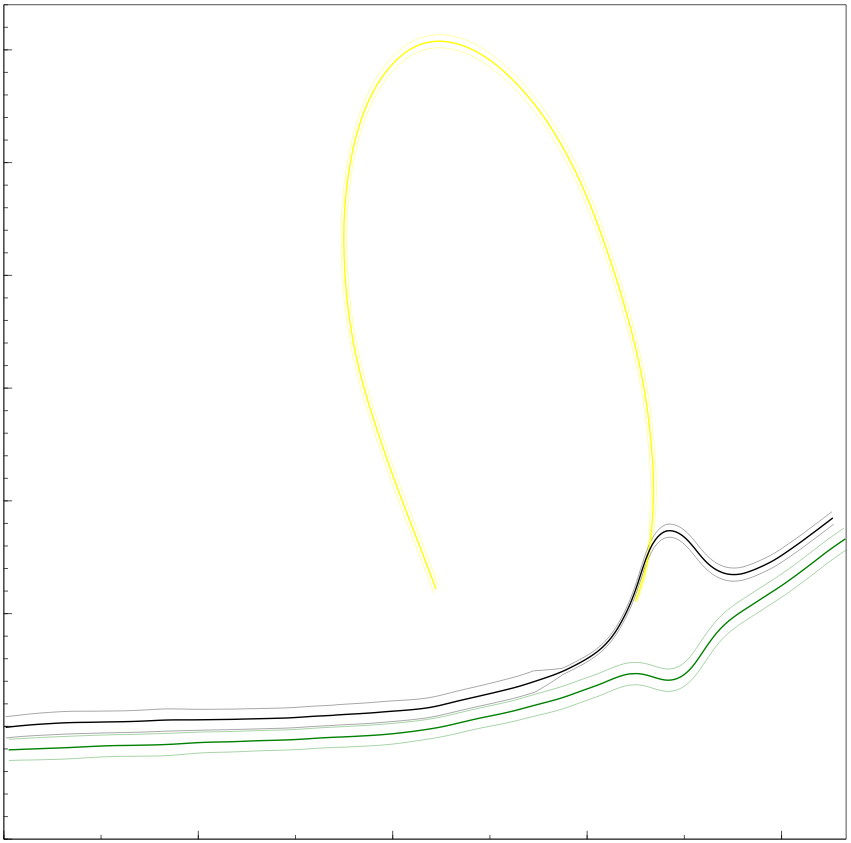
\includegraphics[align=c, width=0.29\linewidth]{resources/img/results/Steinheim/improvedLanes_Steinheim}
    }}
    \caption{Ergebnisse Spur-Geometrie-Bestimmung}
    \label{fig:results_laneGeometries}
\end{figure}

Anhand der abgebildeten Spurgeometrien ist ersichtlich, dass das in Abschnitt \ref{cha:lane_definition}
beschriebene Verfahren gute Ergebnisse in unterschiedlichen Situationen liefert.
Plot a) zeigt die Spur-Geometrien, welche im Fall des Datensatzes der Heilbronner-Straße bestimmt werden.
Für jedes Spurcluster, welches in Abbildung \ref{fig:results_clusters} a) zu sehen ist, wurde eine Geometrie erstellt.
Es ist zudem zu sehen, dass die Fahrspuren partitioniert wurden, um Überlagerungen zu vermeiden.
Plot b) veranschaulicht, dass Spurgeometrien auch korrekt bestimmt werden, wenn in einer Aufnahme
Fahrbahnerweiterung existieren.
Anhand von Plot c), welcher die für den Datensatz \textit{Steinheim} extrahierten Spur-Geometrien zeigt, wird
außerdem deutlich, dass auch die Geometrien kreisförmiger Fahrspuren und Kreisverkehre bestimmt werden können.

Zwei Probleme, welche bei der Bestimmung der Spur-Geometrien auftreten können, sind in Abbildung
\ref{fig:results_defekts_laneGeos} dargestellt. In diesem Fall stammen die Beispiele aus den Geometrien
des Datensatzes \textit{Heilbronner-Straße}.

\begin{figure}[H]
    \centering
    \subfloat[Problem Partitionierung]{{
        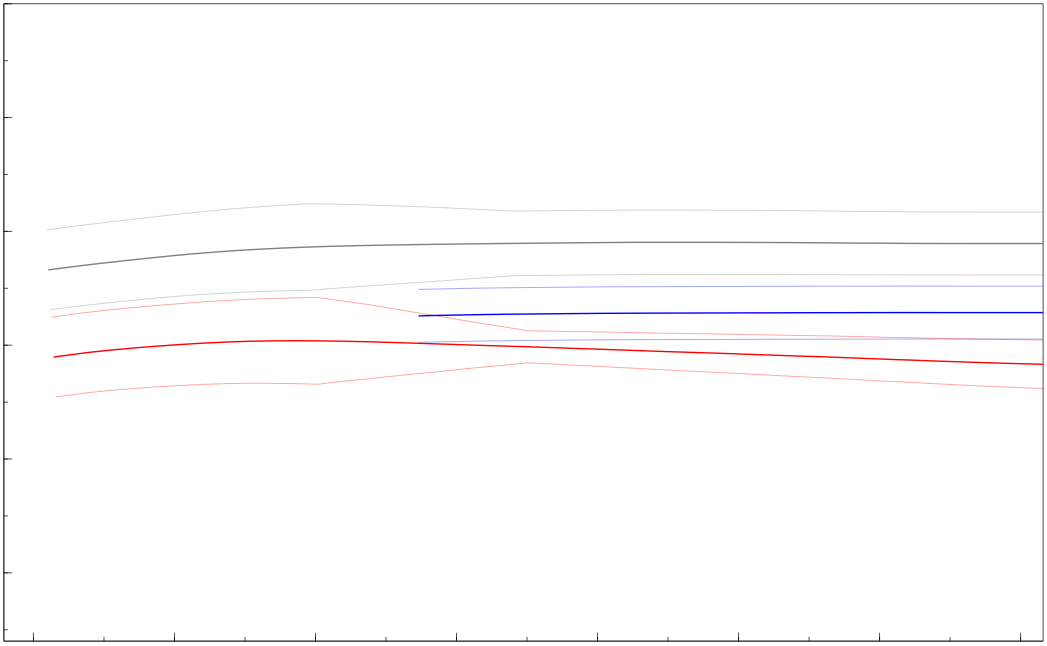
\includegraphics[align=c, width=0.4\linewidth]{resources/img/results/Defekte/Defekt_Part}
    }}
    \qquad \qquad
    \subfloat[Problem Spurbreite]{{
        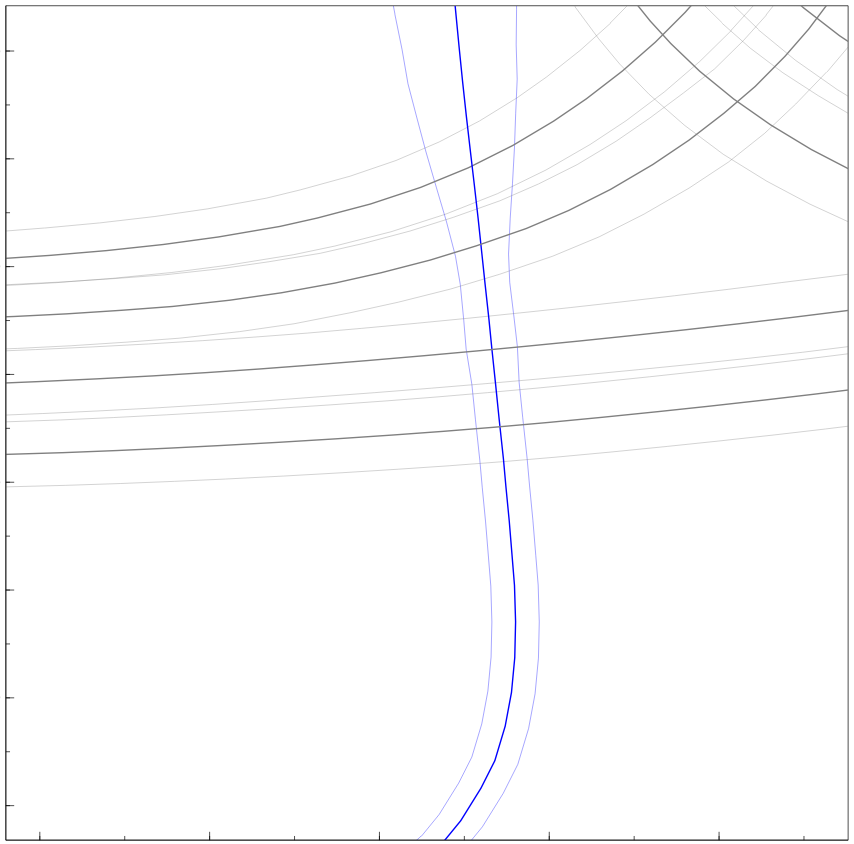
\includegraphics[align=c, width=0.3\linewidth]{resources/img/results/Defekte/Defekt_Width}
    }}
    \caption{Auftretende Probleme in den Spur-Geometrien}
    \label{fig:results_defekts_laneGeos}
\end{figure}

Teil a) der Abbildung zeigt drei Fahrspuren, welche parallel zueinander verlaufen.
Auf dem entsprechenden Staßenabschnitt der Heilbronner-Straße, auf welchem sich die drei Spuren befinden,
verschmälert sich am linken Rand die Fahrbahn und die unterste Spur (rot) geht in die mittlere Spur (blau) über.
Bei der Partitionierung der Spuren sollte daher eigentlich die mittlere Spur vollständig erhalten bleiben
und das Ende der unteren entfernt werden. Wie oben zu sehen ist, wird allerdings die mittlere Spur partitioniert
und die untere bleibt erhalten. Hier trifft der in Abschnitt \ref{sec:real2_lane_partitioning} beschrieben
Algorithmus die ``falsche'' Entscheidung.

In Abbildung \ref{fig:results_defekts_laneGeos} b) ist zu sehen, dass die blau markierte Spur
in ihrem Verlauf nach unten hin schmäler wird. Dies entspricht nicht ihrem realen Verlauf auf der Straße.
Diese Schmälerung tritt auf, da der Algorithmus zur Optimierung der Spurbreiten (siehe Abschnitt \ref{sec:real2_lane_geo_opt})
auf einer bestimmten Höhe den Abstand zur falschen Spur zur Neu-Berechnung der Breite verwendet.
Die fehlerhafte Breite wird anschließend für den Rest der Spur weiterverwendet.

Die beiden oben abgebildeten und beschrieben Fehler treten in ähnlicher Art gelegentlich auf. Der Grund hierfür
ist, dass es sowohl im Fall der Spur-Partitionierung als auch im Fall der Bestimmung der Spur-Breite sehr schwierig ist,
ein Verfahren zu definieren, welches in allen Fällen die ``richtige'' Entscheidung trifft.
Ein menschlicher Betrachter kann bei der Überlagerung zweier Spuren zwar meist intuitiv feststellen, welche
partitioniert werden muss, einem Algorithmus dies beizubringen ist allerdings schwierig.

Die verwendeten Ansätze liefern in der Mehrzahl der Fälle allerdings die ``richtige'' Lösung, was in diesem Anwendungsszenario
absolut ausreichend ist. Gerade bei der Partitionierung der Spuren gibt es oft auch kein eindeutiges ``richtig'' und ``falsch''.
Welche Spur erhalten bleiben soll, ist häufig Interpretationssache. Daher, und da die oben beschriebenen ``Fehler''
leicht über die Oberfläche der \textit{Vehicle-Tracker} Anwendung korrigiert werden können, wurden die verwendeten
Algorithmen hier nicht weiter angepasst.

\section{Ergebnisse der Spurerkennung}

Nachdem in den obigen Abschnitten auf die Fähigkeiten und Probleme der drei Hauptschritte des
Spurerkennungs-Algorithmus eingegangen wurde, werden nun Ergebnisse in Form von Screenshots vorgestellt.
In ihnen sind die automatisch erkannten und erstellten Spuren in der Anwendung \textit{Vehicle-Tracker} zu sehen.

Die zwei ersten Screenshots, welche in Abbildung \ref{fig:results_lanes1} dargestellt sind, zeigen die erkannten
Spuren im Fall der Datensätze \textit{Entennest} und \textit{Düsseldorf}.
Anhand der Aufnahmen ist ersichtlich, dass die erstellten Fahrspuren gut mit den realen Verläufen der
Spuren auf der Fahrbahn übereinstimmen.
Dies gilt auch im Fall des Datensatzes \textit{Düsseldorf}, obwohl die hier detektierten Fahrzeugpositionen
aufgrund des niedrigen Aufnahmewinkels nicht immer in der Nähe der Spurmitte liegen.
% TODO: Evtl. Grund fehlende Spur Düsseldorf

\begin{figure}[H]
    \centering
    \subfloat[Fahrspuren Entennest]{{
        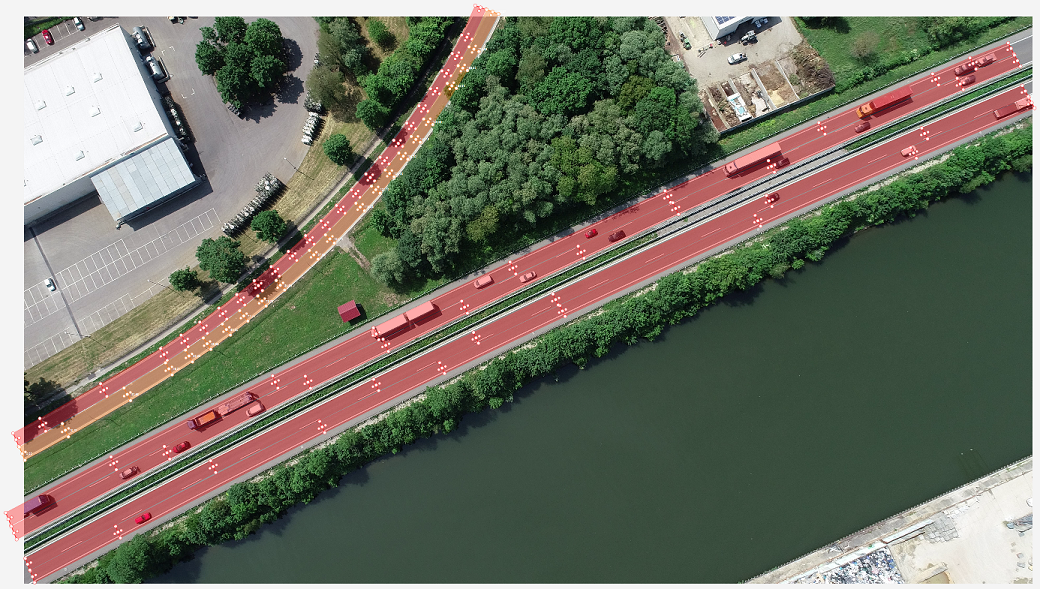
\includegraphics[align=c, width=0.5\linewidth]{resources/img/results/Lanes/Entennest_Lanes}
    }}
    \subfloat[Fahrspuren Düsseldorf]{{
        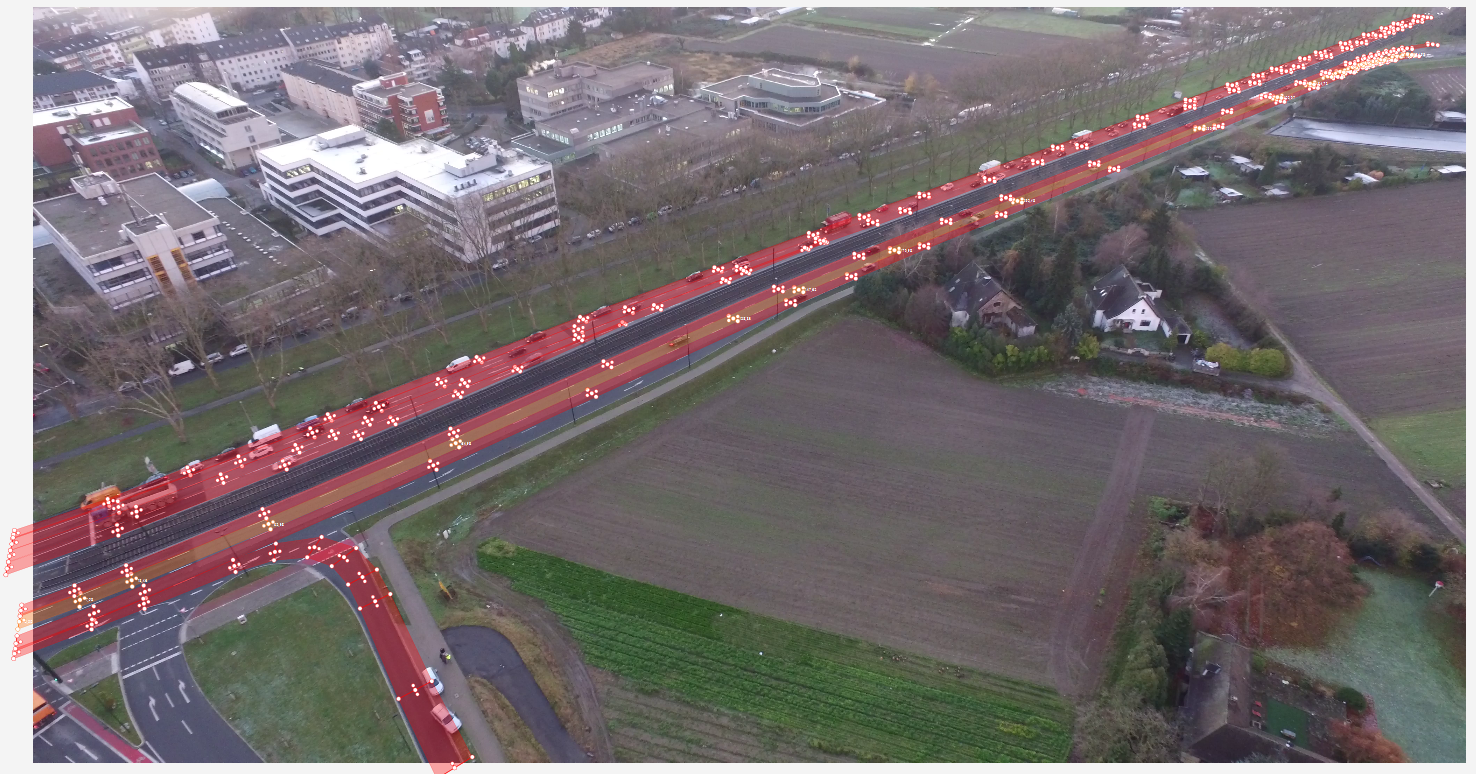
\includegraphics[align=c, width=0.5\linewidth]{resources/img/results/Lanes/Duesseldorf_Lanes}
    }}
    \caption{Erkannte Fahrspuren auf geraden Straßenabschnitten}
    \label{fig:results_lanes1}
\end{figure}

In Abbildung \ref{fig:results_lanes2} sind die erkannten Spuren der Datensätze \textit{Neckartor} und \textit{Heilbronner-Straße}
dargestellt. Auch hier stimmen die Spur-Geometrien gut mit den realen Spur-Ausmaßen überein. Zudem wird deutlich,
dass sowohl die Partitionierung der Spuren als auch das angleichen benachbarter Spurenden die gewünschten Resultate liefern.
Im Fall der Heilbronner-Straße ist nun auch zu sehen, dass im unteren rechten Bereich keine Spur erkannt wird.
Der Grund hierfür wurde in Abschnitt \ref{sec:results_eval_clustering} beschrieben.

\begin{figure}[H]
    \centering
    \subfloat[Fahrspuren Neckartor]{{
        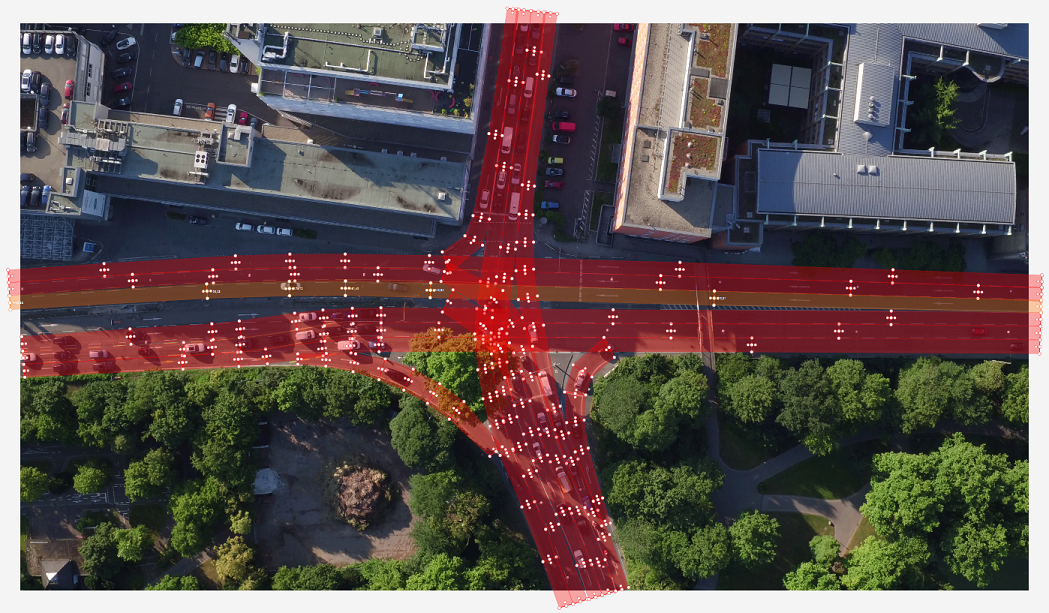
\includegraphics[align=c, width=0.5\linewidth]{resources/img/results/Lanes/Neckartor_Lanes}
    }}
    \subfloat[Fahrspuren Heilbronner-Straße]{{
        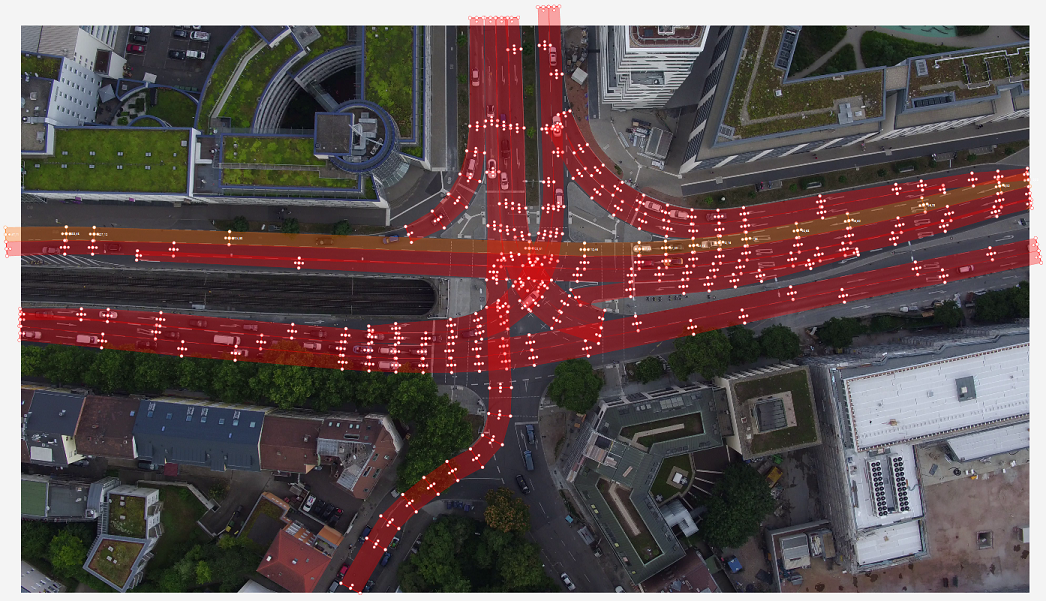
\includegraphics[align=c, width=0.5\linewidth]{resources/img/results/Lanes/Heilbronner_Lanes}
    }}
    \caption{Erkannte Fahrspuren auf Kreuzungen}
    \label{fig:results_lanes2}
\end{figure}

Der Screenshot in Abbildung \ref{fig:results_lanes3} zeigt die erkannten Fahrspuren im Datensatz \textit{Steinheim}.
Dieses Beispiel zeigt, dass Fahrspuren auch in Straßenabschnitten mit Kreisverkehren oder kreisförmigen Spuren
erkannt werden. Auch hier stimmen, trotz des niedrigen Aufnahmewinkels, die Fahrspuren weitestgehend
mit den realen Fahrbahnverläufen überein.

% TODO: wenn finale Aufnahe vorliegt, weiter ausführen

\begin{figure}[H]
    \centering
    \subfloat[Fahrspuren Steinheim]{{
        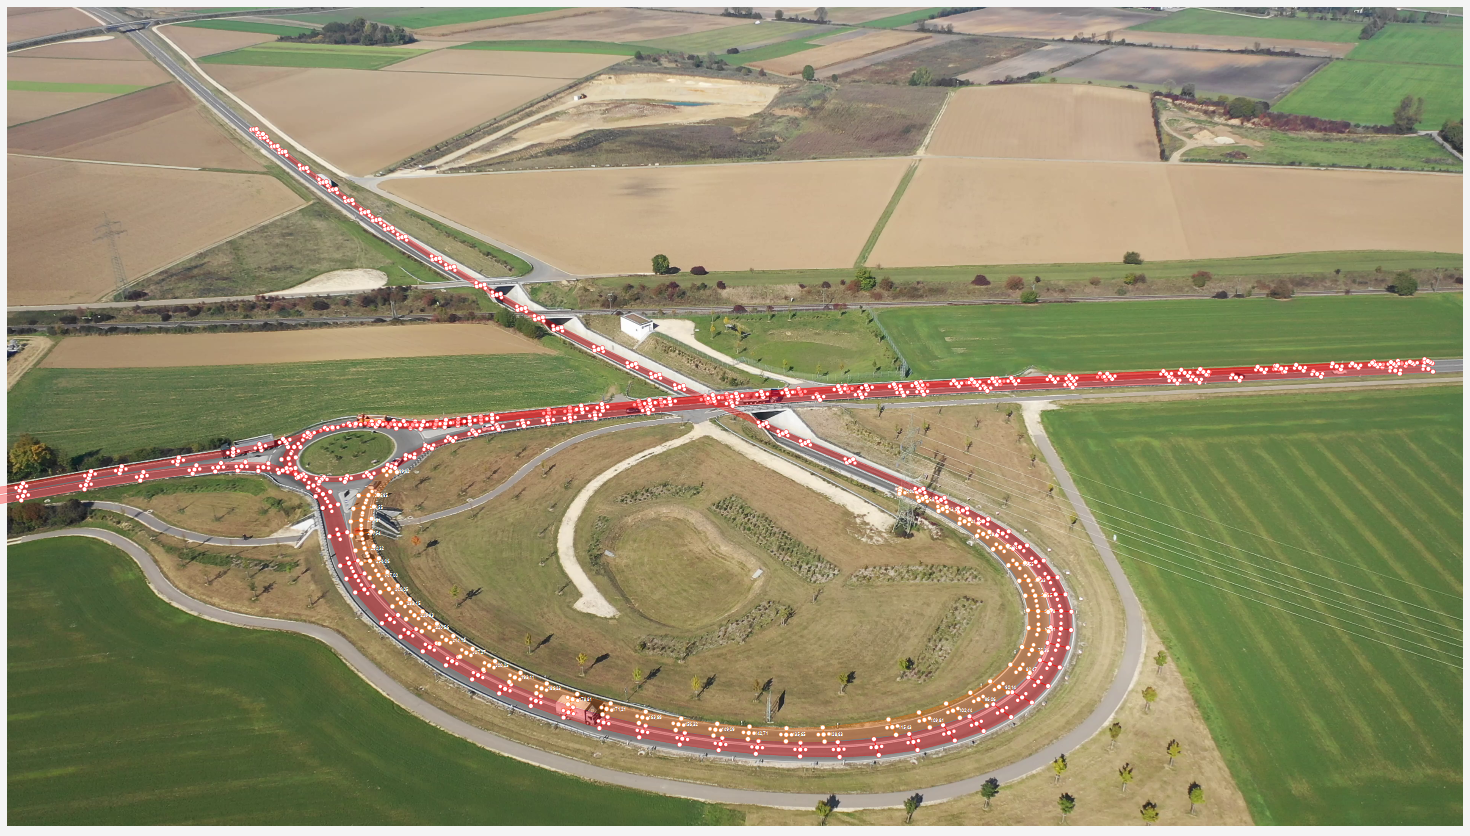
\includegraphics[align=c, width=0.5\linewidth]{resources/img/results/Lanes/Steinheim_Lanes}
    }}
    \caption{Erkannte Fahrspuren Kreisverkehr}
    \label{fig:results_lanes3}
\end{figure}

% TODO: evlt mehr bilder
% TODO: Schluss